\documentclass[12pt]{article}
\usepackage{graphicx}
\usepackage{amsmath}
\usepackage{amsfonts}
\usepackage{subfigure}
\usepackage{fullpage}
\usepackage{footnote}
\usepackage[backend=biber, sorting=nyt]{biblatex}
\bibliography{oralrefs}
\usepackage{setspace}
\doublespace
%\onehalfspace
\usepackage[font=footnotesize, labelfont=bf]{caption}
\begin{document}
\author{Michael Crumrine}
\title{CMB polarization with the Bicep and Keck experiments}
\maketitle



\section{Introduction}

\subsection{A Brief History of Inflation}
The modern study of cosmology began in 1915 with Einstein's development of the general
theory of Relativity \cite{cite:Einstein}. By combining the Einstein Field
Equations with the assumptions of a homogeneous and isotropic universe,
Friedmann developed a cosmological model which forms the core of the standard
model of cosmology\cite{cite:Friedmann}. Hubble's observations in the 1930s
showed an expanding universe\cite{cite:Hubble} providing the first evidence
for a Big Bang origin. This was further supported by the detection of the
Cosmic Microwave Background by Penzias and Wilson in 1965\cite{cite:Penzias}.


Increasing experimental precision revealed a uniform CMB and isotropic
universe on scales exceeding the size of the horizon predicted by
Friedmann cosmological models. In 1981 Guth suggested a small period of
exponential expansion to solve these two problems. This theory of inflation
has since seen further success in explaining the growth of cosmic structures
and the lack of observed magnetic monopoles but has been criticized due to its
need for fine-tuned initial conditions.


\subsection{Origins of the CMB}
One of the most successful predictions of inflation is the presence of a near
uniform isotropic photon source known as the Cosmic Microwave Background
(CMB).The CMB has the near uniform temperature spectrum of a 2.73K blackbody
and is the source of the oldest photons in the universe. In the hot big bang, the
early universe was an energetic plasma in which photons scattered continuously
from free protons and electrons which prevented propagation over large
distances. As the universe expanded, the temperature of this plasma decreased
adiabatically until the free electrons and protons could combine to form
neutral Hydrogen. After this era of recombination about 380,000 years after
the big bang, the photons decoupled from the plasma and began free streaming
through the universe, redshifting due to continued expansion. We observe
these photons as a 2D "surface of last scattering". 

\section{Science with the CMB}

\subsection{Mapping the CMB}
Precision cosmology experiments have shown that the CMB is not truly uniform.
Results from COBE in 1992\cite{cite:COBE} showed the CMB to have a nearly
isotropic temperature spectrum corresponding to a 2.73K blackbody but with
fluctuations on the order of 10 $\mu$K. We examine these temperature
perturbations with the spherical harmonics:


\begin{equation}
	\delta T(\theta,\phi) = \sum _{m=-\ell} ^\ell \sum _{\ell=0} ^\infty
	a_{\ell m}Y_{\ell m}(\theta,\phi)
\end{equation}


Although this decomposition is a powerful tool, the universe is isotropic only
in a statistical sense and we therefore cannot predict any individual $a_{\ell
m}$. We instead take an average over $m$ for a given $\ell$ to form the
angular power spectrum:

\begin{equation}
	C_{\ell} = \frac{1}{2\ell +1}\sum _{m=-\ell} ^\ell |a_{\ell m}|^2
\end{equation}


The temperature power spectrum shown in Figure \ref{fig:temp_aps} contains
much of the information concerning the geometry, evolution, and composition of
our universe.
%The simple $\Lambda$CDM model is based on the six parameters
%shown in Table \ref{table:lcdm6par}. 
\begin{figure}
	\center
	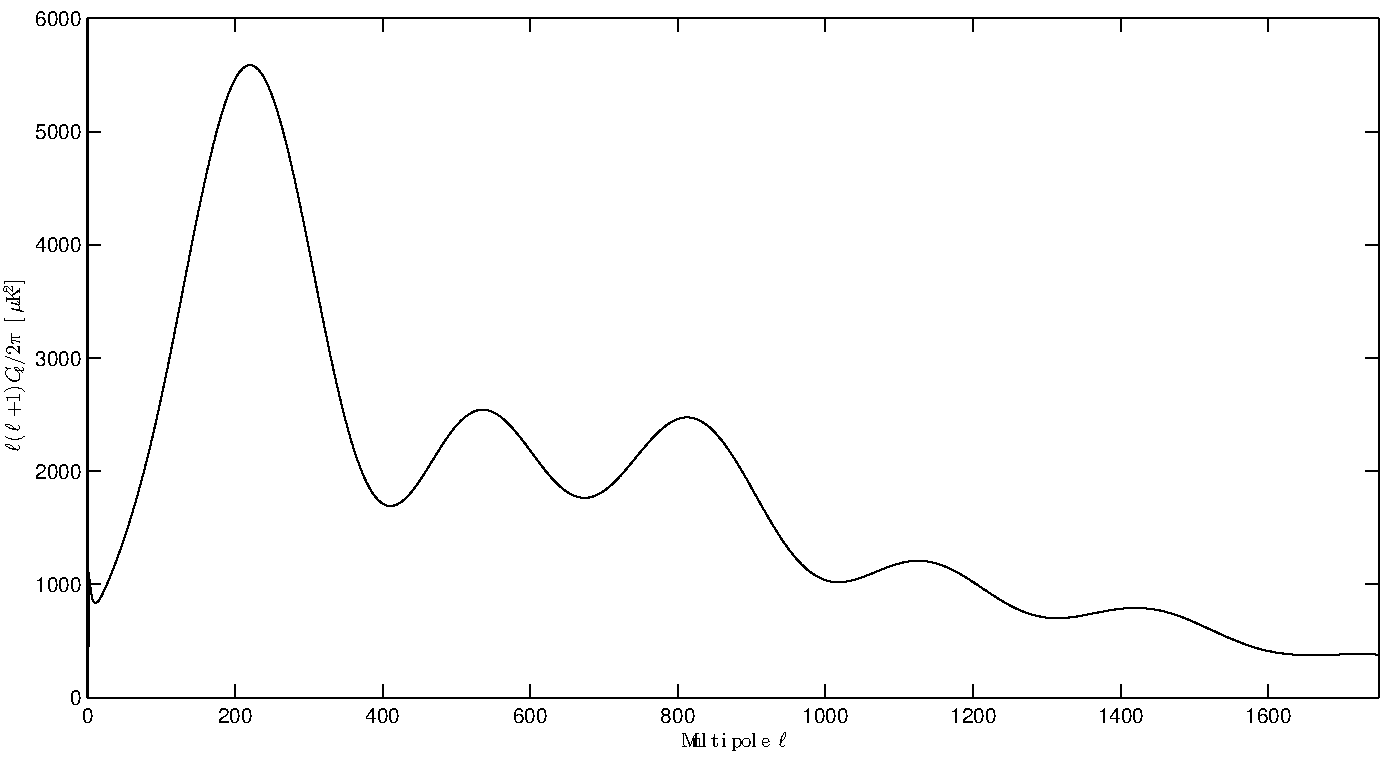
\includegraphics[width=.8\textwidth]{temp_aps.pdf}
	\caption{The temperature power spectrum of the CMB. The primary and
	acoustic peaks can be used to constrain cosmological parameters that
	describe the geometry, evolution and composition of our universe.}
	\label{fig:temp_aps}

\end{figure}

%\subsection{The 6 Parameter Model}

%\begin{table}
%	\center
%\begin{tabular}{|l|l|l|}
%	\hline
%	Parameter & Symbol & Value \\ \hline \hline
%	Baryon Density & $h^2\Omega _b$ &  $0.02240$\\ \hline
%	Cold Dark Matter Density & $h^2\Omega _m$ & $0.1146$ \\ \hline
%	Dark Energy Density ($w=-1$) & $\Omega _\Lambda$ & $0.7181$ \\ \hline
%	Scalar Spectral Index & $n_s$ & $0.9646$ \\ \hline
%	Curvature Fluctuation Amplitude $k_0=0.002$ & $\Delta _\mathcal{R} ^2$ & $2.43
%	\times 10^{-9}$\\ \hline
%	Reionization Optical Depth & $\tau$ & $0.0800$\\ \hline
%\end{tabular}
%	\caption{The six parameters in the simple $\Lambda$CDM
%	cosmological model as shown in the WMAP 9 year results\cite{cite:WMAP9}}
%	\label{table:lcdm6par}
%\end{table}
%
%The first three parameters in Table \ref{table:lcdm6par} - $h^2\Omega_b$, $h^2\Omega _c$, and $\Omega
%_\Lambda$ - describe relative contribution to the composition of our universe
%from baryons, cold dark matter, and dark energy respectively. The matter to
%baryon ratio is related to the size of the first three peaks of the
%Temperature power spectrum in Figure \ref{fig:temp_aps}. The scalar spectral
%index $n_s$ measures the deviation of the power spectrum from the
%scale-invariant case.  The curvature fluctuation amplitude $\Delta
%_\mathcal{R} ^2$ is a
%measure of curvature fluctuation at different angular scales. Finally, the
%reionization optical depth can be used to estimate the damping of CMB
%fluctuations due to the reionization of cosmic baryons which turns the
%universe more opaque for CMB photons.
%WMAP 5yr paper has information on these parameters, so does Dark Universe

%These 6 parameters are largely degenerate with each other in CMB studies
%alone. To break the degeneracies, CMB data is often combined with data from
%other cosmological studies which can set constraints independent of the CMB.
%Studies of Type Ia supernovae use well characterized spectral emissions to create a
%cosmic distance ladder which can constrain the Hubble constant and place
%independent constraints on the composition of the universe. An independent
%measure of these parameters can be made by studying Baryon Acoustic
%Oscillations. The attraction of matter by a primordial overdensity leads to
%increased heat and a large outward pressure. These pressure waves of baryons
%were left behind at fixed radii after photon decoupling leaving a large
%overdensity at the sound horizon. By comparing the overdensities in the CMB
%with the distribution of modern galaxies, BAO places constraints on cosmic
%expansion independent from those set by CMB or supernovae studies.






\subsection{Polarization Anisotropies}
In addition to the temperature anisotropies CMB photons are partially
polarized due to Thompson scattering in a non-uniform temperature field. This
CMB polarization was predicted at the $\approx 10\%$ level by Bond et al
\cite{cite:Bond} and first detected by DASI in 2002 \cite{cite:DASI}. Polnarev
\cite{cite:Polnarev} realized that an inflationary period would imprint an
additional polarization signal on the CMB due to the production of
gravitational waves. 

This inflationary gravitational wave (IGW) signal is expected to be orders of
magnitude fainter than the signal due to Thompson scattering and difficult to
separate in the Stokes parameter space conventionally used when studying
linearly polarized light. It was shown by Kamionkowski et al
\cite{cite:Kamionkowski} that the polarization could instead be parameterized
by a gradient (E-mode) and curl (B-mode) component. The signal produced by
Thompson scattering occurs in the presence of a temperature quadrupole and
follows the temperature gradients of the hot plasma at recombination. It can
therefore produce only E-modes. The tensor perturbations due to passing
gravitational waves are not restricted in this way and can thus generate both
E and B modes. The signal produced by these two methods is characterised by
the tensor to scalar ration $r$. 

In addition to the temperature power spectrum, we can then examine the
E, B power spectrum as well as cross correlations between the temperature and
polarization power spectra. Figure \ref{fig:theory_aps} shows the
theoretical power spectra of CMB perturbations in the $\Lambda$CDM standard
model of Cosmology with the addition of an $r=0.1$ IGW B-mode signal. 



\begin{figure}[ht]
	\center
	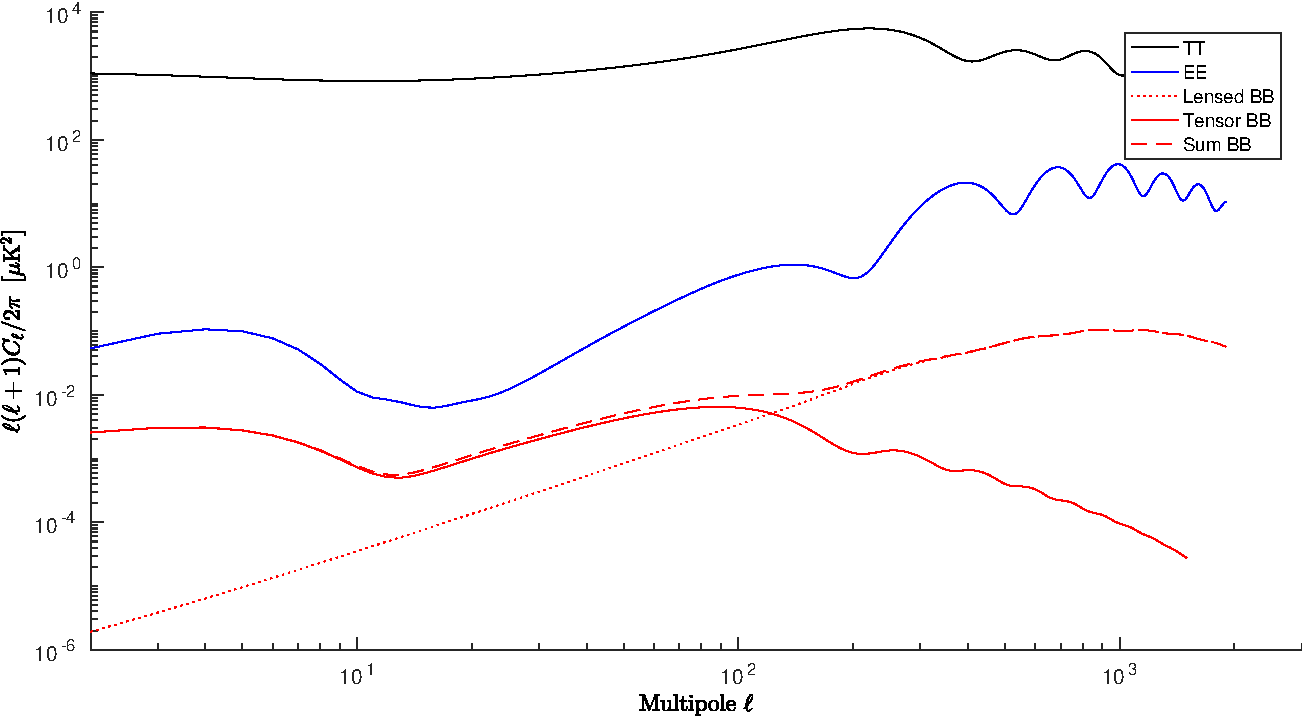
\includegraphics[width=.8\textwidth]{theory_aps.pdf}
	\caption{The CMB power spectrum of the $\Lambda$CDM standard model of
	cosmology as calculated by CAMB using parameters from Planck 2013. The
	temperature anisotropies (black) contain orders of magnitude more power
	than the E-mode (blue) and B-mode (red) polarization anisotropies. The BB
	spectrum is split into a lensing component (dotted) and a tensor component
	(solid) plotted at the $r=0.1$ level.}
	\label{fig:theory_aps}

\end{figure}


\subsection{Constraints on Inflation}
Although the theory of inflation provides an attractive solution to a number
of problems with the standard big bang cosmology, the exact physics of
inflation are still undetermined. The favored theory of slow roll inflation
proposes a scalar field $\phi$ in which the potential of the field dominates
over its kinetic energy. There mare many possible potentials which fit the
mathematical requirements of inflation theory which yield a range of values
for the tensor to scalar ratio. By continuing to push the constraints on $r$
we restrict the possible potentials of this scalar field. A summary of current
restrictions on $r$ and $n_s$ which depends on the slow roll parameters is
shown in Figure \ref{fig:status}. The Bicep / Keck constraints heavily
disfavor the $\phi ^2$ model but still allow for other models which have
$r<0.1$


\begin{figure}
	\resizebox{0.63\textwidth}{!}{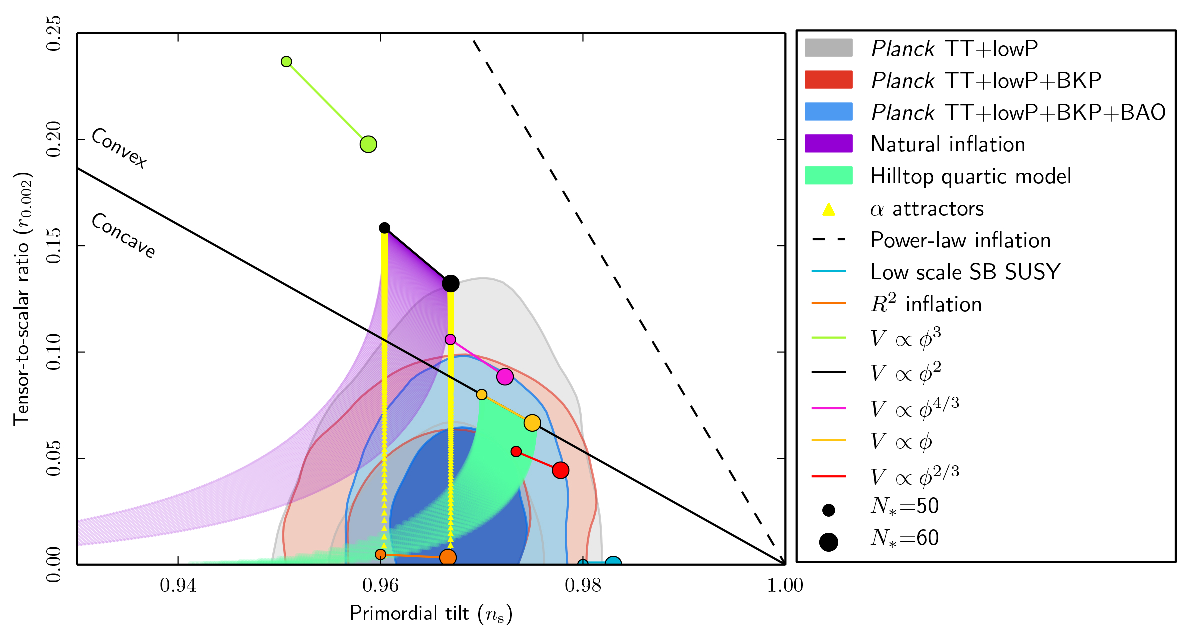
\includegraphics{planck2015XXfig54.pdf}}
	\resizebox{0.36\textwidth}{!}{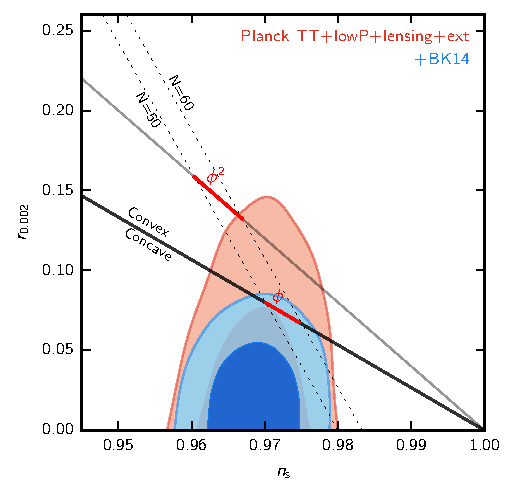
\includegraphics{bk14fig7.pdf}}
	\caption{Left: Reproduced from Planck 2015 XX: "Constraints on
	Inflation"\cite{PlanckXX}
	shows theoretical predictions for select inflationary models in
	the $n_s$,$r$ parameter space and current constraints on those
	parameters. The two dots correspond to different numbers of e-folds.
	Right: Reproduced from BK-VI \cite{BK6} showing improved constraints in this
	parameter space from the latest Bicep / Keck data including a 95GHz band.}
	\label{fig:status}
\end{figure}


\section{The Bicep and Keck Program}
The Bicep/Keck experiments are a staged series of small aperture ground based
telescopes which aim to produce extremely deep degree-scale polarization maps
of the CMB. The high systematics control and long integration time have
enabled Bicep and Keck to set the strictest limits on inflationary
gravitational wave B-mode signal to date. Current published B-mode
measurements are shown in Figure \ref{fig:BK_vs_world}.

\begin{figure}
	\center
	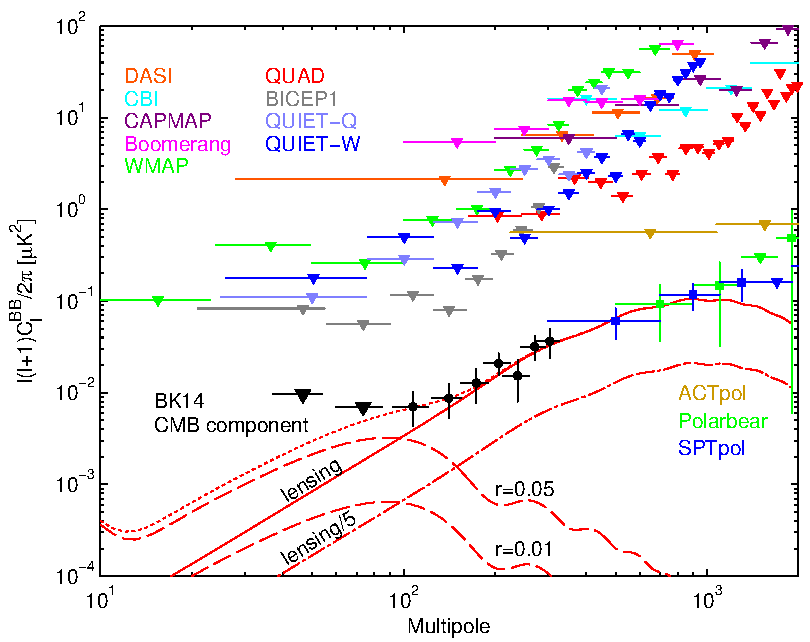
\includegraphics[width=.7\textwidth]{bk14_vs_world.pdf}
	\caption{Published B-mode polarization measurements of the CMB.
	Theoretical predictions for lensing B-modes (solid red) and IGW B-modes
	(dashed red) for two values of r are shown. The SPTpol, Polarbear and
	Bicep/Keck experiments have all recently detected the B-mode lensing
	signal. Bicep and Keck are currently alone in probing large
	angular scales for the IGW B-mode signal}
	\label{fig:BK_vs_world}
\end{figure}


Each generation of receiver builds on the experience gained from
the previous generation while pushing deeper in sensitivity.
Bicep1 was deployed to the south pole in 2006 and used 98 feedhorn coupled
bolometers observing at 100GHz and 150GHz. Over three observing seasons the
strategies developed for observation, calibration and systematics control
proved the efficacy of small aperture refractors for CMB polarization studies
and established the leading upper bounds on inflation at $r<0.70$
\cite{cite:Bicep1}.

Building on the techniques developed with its predecessor, Bicep2 replaced
Bicep1 in 2009. It exchanged feedhorn coupled bolometers for antenna-coupled
transition edge sensor (TES) bolometer arrays developed at JPL which have been
used in every subsequent telescope in the series. Concentrating its observing
power at 150GHz, in March 2014 Bicep2 announced a detection of excess signal
in its observing band consistent with an IGW signal of $r=0.2$\cite{cite:BK1}.
However, the interpretation of this excess as IGW signal relied heavily on
models of polarized dust emission which had not been highly constrained at the
time. Later that year new high frequency maps from the Planck experiment
indicated that the dust models had underestimated polarized emission in the
faintest sky regions \cite{cite:PlanckXIX}. A joint analysis with Planck and
cross correlation between the Planck 353GHz and Bicep2 150GHz maps showed that
a substantial part of the observed excess in Bicep2 was due to polarized dust
emissions \cite{cite:BKP}. This joint analysis established a new upper limit
of $r<0.12$

The Keck Array deployed to the south pole in 2012 with five 150GHz receivers
similar to Bicep2. These additional receivers confirmed the excess signal
found with Bicep2 and contributed to the March 2014 results. In addition to
extending the Bicep2 survey depth at 150GHz the Keck array has extended
observations into three other observing bands at 95GHz, 220GHz and 270GHz. The
extension into other frequencies harnesses the Bicep/Keck program's proven
capability to make deep maps to further constrain galactic foregrounds and
refine the models of polarized dust emission. The Keck array is in its final
observing season with four receivers in the 220GHz band and one at 270GHz.

In the fall of 2014 Bicep3 was deployed at the south pole to run concurrently
with the Keck array. Bicep3 vastly expands the design of the Bicep2 instrument with a
focal plane containing 2500 detectors in the 95GHz band, almost 10x the 288
detectors of a Keck style 95GHz receiver. Bicep3 serves as our prototype
instrument leading to the eventual replacement of the Keck array with Bicep
array.

The Bicep array is a funded experiment which will replace the Keck Array for
multifrequency observations. Using the more powerful Bicep3 style receivers,
Bicep array will field three receivers centered at 35GHz, 95GHz, and 150GHz
along with a dual band 220/270GHz receiver. The new 35GHz receiver will
heavily constrain galactic synchrotron radiation past the upper limits set by
WMAP's 23GHZ band while the increased sensitivity at higher frequencies will
allow for better constraints on dust emissions at frequencies closer to our
other bands than the Planck 353GHz data.


\begin{figure}
	\center
	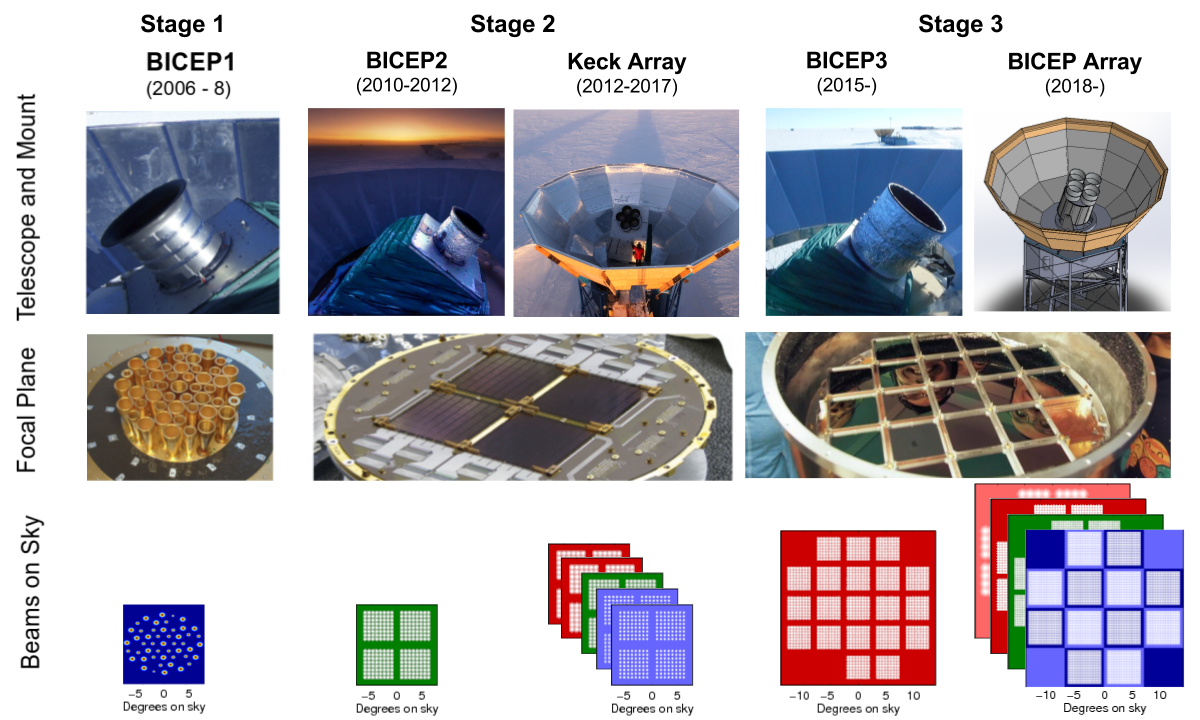
\includegraphics[width=.8\textwidth]{BK_progression.png}
	\caption{The progression of the Bicep/Keck program from Bicep1 to Bicep
	Array. The bottom row shows the beam patterns of the focal planes on the
	sky. With the exception of Bicep1 the focal plane colors correspond to
	band centers of: 35GHz - pink, 95GHz - red, 150GHz - green, 220 GHz -
	light blue, 270GHz - dark blue.}
	\label{fig:BK_progression}
\end{figure}




\section{Multifrequency Observations}

CMB polarization experiments must be able to separate polarized foreground
signals from those imprinted on the CMB. Although these signals can be
minimized by selection of observing area their emissions must be constrained
and accounted for. As shown by the 2014 joint analysis between Bicep2/Keck and
Planck, constraints on these models have significant impact on the
interpretation of any observed excess signal. By expanding observations into
multiple frequencies, the Keck array has further constrained these dust
emissions as well as emissions due to galactic synchrotron as shown in Figure
\ref{fig:noilev}.
\begin{figure}
	\center
	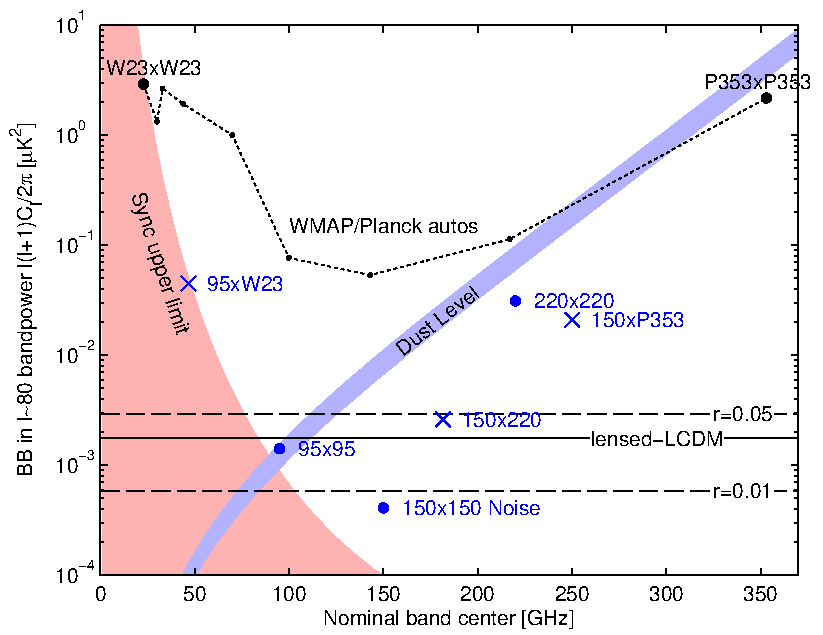
\includegraphics[width=.7\textwidth]{noilev_bk15.pdf}
	\caption{Noise levels in the Bicep/Keck combined observations through the
	2015 observing season. The shaded regions show constraints on the signal
	level of galactic foregrounds and signal levels corresponding to select values
	of $r$ are shown at the bottom. All values are shown in the $\ell=80$
	bandpower where the IGW signal is expected to be maximal.}
	\label{fig:noilev}
\end{figure}

\subsection{Polarized Dust}
Polarized emissions from galactic dust provide an excess BB signal on top of
that expected from $\Lambda$CDM and gravitational lensing which (although low
in power) are significant compared to the IGW signal. These emissions depend
significantly on frequency, exhibiting a power law like dependence. As shown
in Planck XXII \cite{cite:PlanckXXII} the spectral energy distribution of
galactic dust can be described by a modified blackbody spectrum

\begin{equation}
	I_d=A_d\nu ^\beta B_{\nu}(T_d)
	\label{eq:dust_sed}
\end{equation}

Where $A_d$ is an amplitude at some frequency and $\beta _d > 0$ is the spectral
index of dust emission and $B(T)$ is the standard blackbody spectrum. In order
to fully constrain the dust signal we must complement this intensity
spectrum with a description of the dust's spatial behavior

\begin{equation}
	D_\ell \propto \ell^\alpha
	\label{eq:dust_aps}
\end{equation}

where $D_\ell=C_\ell \frac{\ell(\ell +1)}{2\pi}$. The parameters in these
equations model the dust contribution to polarization signal in our field. As
Equation \ref{eq:dust_sed} shows this signal is brighter at higher
frequencies. We therefore use the Planck 353GHz maps to set these dust
parameters and extrapolate to our observed frequencies. This necessarily means
that any uncertainty contained in the high frequency observations is magnified
due to the power law behavior.

Figure \ref{fig:noilev} shows the noise uncertainty and signal levels
the $\ell=80$ bandpower where the IGW signal is expected to peak. The low 150x150
noise allows us to detect excess signal with high significance. However, the high P353xP353
noise as compared to dust signal does not provide significant enough
constraining power to separate dust signal from potential IGW signal in the
150GHz band. The 220x220 point shows preliminary numbers from our 2015
observing season in which the Keck array operated with two 220GHz receivers
and provides similar constraining power to the Planck 353GHz data while being
closer to our main observing bands. Two additional 220GHz receivers were added
for the 2016 observing season and observations at 270GHz will begin in the
current 2017 season. These observations will allow us to produce continually
improving constraints on dust in our field.
\subsection{Galactic Synchrotron}
An upper limit for an additional foreground signal is shown in Figure
\ref{fig:noilev}. Rather than increasing in intensity at higher frequencies,
polarized emissions from galactic synchrotron radiation are strongest at low
frequencies. We model synchrotron emission intensity as
\begin{equation}
	I_\nu = A_s \nu^{\beta _s}
	\label{eq:synch_sed}
\end{equation}

where $\beta _s < 0$ describes the fall off in intensity with frequency and
$A_s$ is the amplitude. The angular power spectrum of galactic synchrotron
follows the same form as dust (Equation \ref{eq:dust_aps}). The points shown
in Figure \ref{fig:noilev} mark the upper limit of synchrotron emissions as
the noise level of current observations in these bands is not sufficient for
detection. Models of the contribution due to synchrotron do not predict
significant contamination at frequencies upwards of 150GHz due to the strong
frequency dependence.

%Look at PIP XXX - might give more information on exactly what this beta
%parameter is. Seems like it might vary with sky patch according to BKP

\section{Bicep Array}

\subsection{Experiment Overview}
Bicep Array will deploy four Bicep3 style receivers in four frequency bands
with first light expected in 2019. Building on the success of previous
experiments, Bicep Array will continue to use the antenna coupled transition
edge sensor (TES) bolometers developed by JPL. These detectors leverage the strong
temperature-dependence of superconductors near their transition point to
detect extremely faint signals. The signal from these bolometers is then
amplified by a series array of superconducting quantum interference devices
(SQUIDs). We use cold optics to minimize the out of band extraneous signal
incident on our detectors.

Each Bicep array receiver will field $\approx$ 10 time the detectors of a Keck
receiver in the same band. The additional increase in aperture from 26cm to
55cm will quickly push sensitivity to synchrotron with Bicep Array's new band
and continue to push sensitivity in our deepest 95GHz and 150GHz bands.
Projections for the sensitivity of the Bicep / Keck experiments including the
Bicep array are shown in Figure \ref{fig:projections}. As we continue to
increase in sensitivity to $r$, the B-mode lensing component will become a
significant contributor to $\sigma _r$. This achromatic foreground cannot be
constrained with multifrequency observations but it can be accounted for via
delensing. Given a high resolution map of the angular deflection field $\Delta
\phi$ of the CMB photons from last scattering to observation it is possible to
undeflect Stokes Q, U maps of polarized signal. The third generation SPT-3G
receiver deployed to the South Pole in late 2016 and will spend a significant
fraction of their time observing the Bicep/Keck sky patch. Using $\phi$ and
Q/U maps provided by SPT-3G will allow us to push $\sigma _r$ below $0.005$.



\begin{figure}[ht]
	\center
	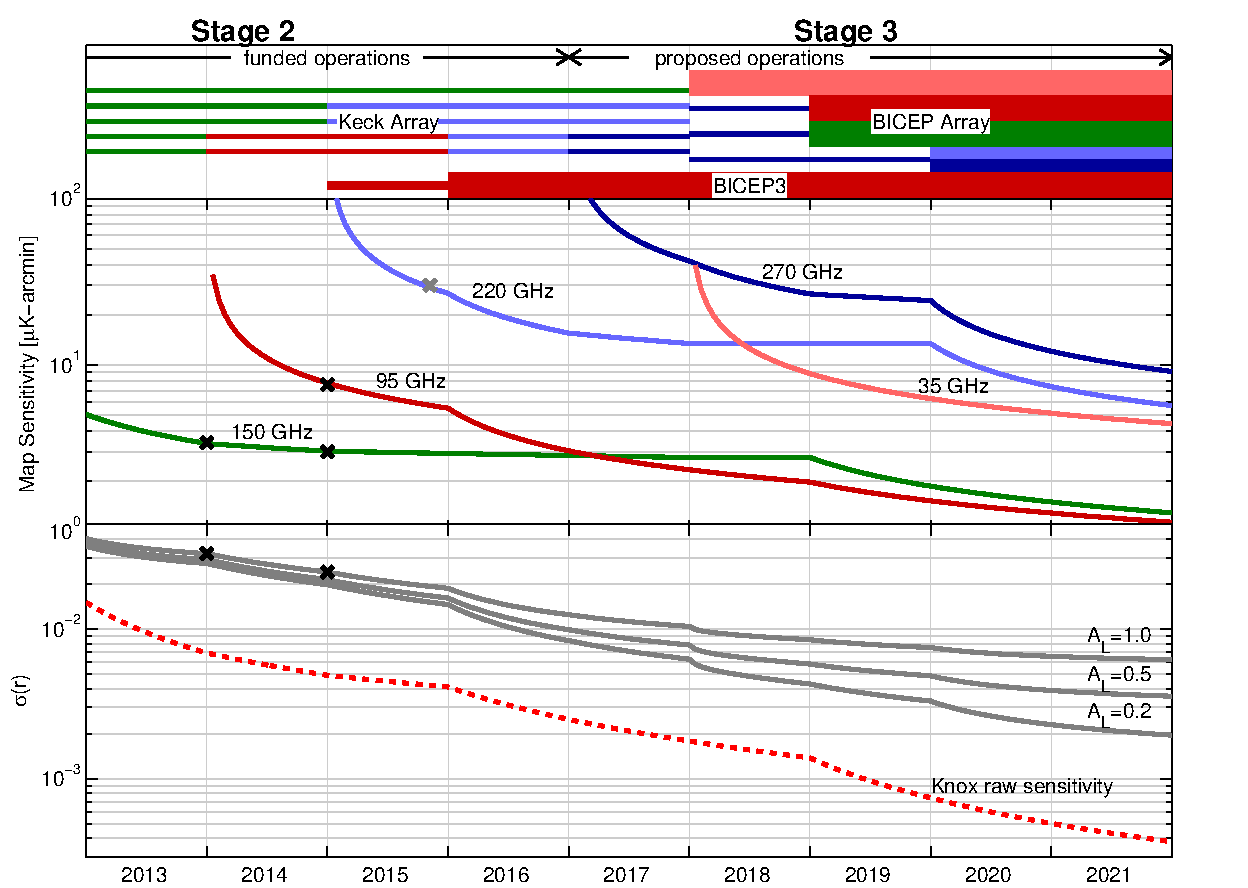
\includegraphics[width=.6\textwidth]{bk_projections.pdf}
	\caption{Projected sensitivity of the ongoing and planned Bicep/Keck
	observational program. The increased throughput of the Bicep array
	receivers will provide increased sensitivity and continue to constrain
	inflation at a rapid rate. \textit{Note: Projections are directly scaled
	from published results and thus include real-world inefficiencies that are
	not reflected in purely theoretical projections. X's mark sensitivities
	achieved in BKP and BK-VI \cite{BK6, cite:BKP}}. Middle: Map depth at each
	frequency as a function of time. Bottom: Sensitivity to $r$ for selected
	levels of delensing efficiency. Performance between $A_L = [0.2, 0.5]$ is
	expected.}
	\label{fig:projections}
\end{figure}


\subsection{Cryogenic Considerations}
The cryogenic operating temperatures of our detector and optics system require
a specially designed housing to thermally isolate the focal plane as much as
possible. As with Keck and Bicep3 the Bicep Array cryostats will consist of a
nested ambient temperature vacuum jacket, a 50K radiation shield, and a 4K
optics tube. This nested approach protects the low temperature optics
from absorbing significant radiative power since $P\propto (T_{H}^4-T_{C}^4)$.
In addition to radiation shielding, there is an additional trade-off between
structural support and heat conduction between the temperature shells. A low
conductive loading may introduce significant deviation in pointing direction
while more structural supports increase the thermal load on the cooling
system. 

\subsection{Thermal Loading}
The cryostat is operated at high vacuum ($\approx 10^{-5}$mTorr) which largely
eliminates conductive loading due to residual gasses. The two largest
contributions are due to conduction across the structural supports and
radiation from higher temperature stages. Of these, the radiation absorbed by
the lower temperature shells has the highest possible contribution. Radiative
heat transfer for cryogenic systems is a well studied subject. We follow
Ekin's textbook on cryogenic engineering to estimate this thermal load
according to:

\begin{equation}
	P=\sigma A_{c} E (T_{h}^4 - T_{c}^4)
	\label{eq:radload}
\end{equation}

where the $h$ and $c$ subscripts denote the hot and cold surfaces
respectively, and $E$ depends on the emissivity of the surfaces as

\begin{equation}
	E=\frac{1}{1/\epsilon _h + 1/\epsilon _c - 1}
\end{equation}

Equation \ref{eq:radload} is valid for parallel plates, and concentric
cylinders assuming specular reflection regime. Table \ref{table:emis} shows
typical emissivities for the materials used in the Bicep Array cryostats. In
addition to the radiative load, the structural supports conduct heat between
the temperature shells according to the Fourier heat transfer law:


\begin{equation}
	\dot{Q}=\int _{T_1} ^{T_2} \frac{A}{L}K(T)dT
\end{equation}

The large temperature change across the support struts require a detailed
knowledge of how the materials' thermal conductivity changes with temperature.
NIST has a collection of thermal conductivity measurements for commonly used
materials in cryogenic design including Aluminum and Titanium. Bicep Array
also uses carbon fiber struts as structural supports, however this material is
non-standardized which makes determining the thermal properties difficult,
especially at high temperatures where few conductivity measurements exist. We
therefore supplement published low temperature measurements with direct
measurements of conducted power in a test cryostat system.




In
estimating the thermal load, our ultimate objective is to ensure that the
innermost 4K shell is able to sufficiently cool the second stage He3 fridge
which is responsible for cooling the TES detectors down to transition. The 50K
stage serves as an intermediate shield that prevents radiation from the 300K
vacuum jacket from directly illuminating any 4K element. However, intercepting
this radiation warms the 50K stage which is also responsible for thermally
sinking an alumina filter. We therefore seek to minimize the thermal load on
both the 50K and 4K stages. 








\begin{table}
	\center
\begin{tabular}{|l|l|}
	\hline
	Rough Aluminum & $\epsilon = 0.07-0.1$ \\
	Polished Aluminum & $\epsilon = 0.04 - 0.06$ \\
	Aluminized Mylar & $\epsilon = 0.035$ \\
	OFHC Copper & $\epsilon = 0.65$ \\ \hline
\end{tabular}
	\caption{Typical emissivity values for materials used in the construction
	of the Bicep Array cryostats.}
	\label{table:emis}
\end{table}






\printbibliography
\end{document}
